\chapter{TỔNG QUAN DỰ ÁN VÀ PHẠM VI TÀI LIỆU}

\begin{ChapterObjectives}
\item Xác định mục đích của bộ tài liệu kỹ thuật cho hệ thống báo cáo năng lượng.
\item Mô tả phạm vi tài liệu, đối tượng sử dụng, và các thành phần cần được duy trì xuyên suốt vòng đời dự án.
\item Cung cấp một chapter mẫu theo phong cách technical manual để nhóm dự án có thể tái sử dụng cho các phần mô tả tính năng, quy tắc nghiệp vụ, và cách tính toán.
\item Minh họa cách trình bày hình, bảng, công thức, và checklist vận hành trong cùng chuẩn LaTeX của dự án.
\end{ChapterObjectives}

\section{Mục đích của tài liệu kỹ thuật}

Tài liệu kỹ thuật của dự án được sử dụng để mô tả hệ thống báo cáo năng lượng theo hướng có thể bảo trì, rà soát, và bàn giao. Nội dung trọng tâm của bộ tài liệu này bao gồm:

\begin{enumerate}[label=-]
\item mô tả mục tiêu và phạm vi của hệ thống;
\item mô tả kiến trúc, luồng dữ liệu, và các thành phần chính;
\item mô tả các tính năng quan trọng theo từng domain như Electricity, Utility, và KPI;
\item ghi nhận các business rules, source-of-truth rules, và nguyên tắc tính toán;
\item mô tả workflow xuất báo cáo và các lưu ý vận hành, phát hành, kiểm tra lỗi.
\end{enumerate}

Cách tổ chức tài liệu này phù hợp với tư duy Documentation-as-Code và vận hành kỹ thuật có kiểm soát thay đổi. Với các dự án ETL hoặc reporting pipeline, tài liệu cần bám sát implementation thực tế thay vì chỉ mô tả ý tưởng tổng quát \cite{ref_kimball,ref_python}.

\section{Phạm vi và đối tượng sử dụng}

Bộ tài liệu này hướng tới các nhóm sử dụng sau:

\begin{enumerate}[label=-]
\item kỹ sư backend và ETL, những người duy trì logic tổng hợp dữ liệu và workflow xuất báo cáo;
\item kỹ sư phụ trách UI hoặc PDF render, những người cần hiểu report context, output artifacts, và layout constraints;
\item người vận hành hệ thống, những người cần biết cách chạy, kiểm tra, và chẩn đoán lỗi pipeline;
\item người rà soát nghiệp vụ, những người cần kiểm tra nguồn dữ liệu, quy tắc KPI, và tính nhất quán của báo cáo.
\end{enumerate}

Phạm vi tài liệu nên tập trung vào các phần có giá trị vận hành dài hạn:

\begin{enumerate}[label=-]
\item project overview;
\item system architecture;
\item data sources và data flow;
\item domain-specific business rules;
\item KPI calculation rules;
\item export conventions, output structure, và release workflow;
\item deployment và operations baseline;
\item troubleshooting và release checklist.
\end{enumerate}

\section{Cấu trúc nội dung khuyến nghị}

Một bộ technical manual cho dự án này nên ưu tiên cấu trúc sau:

\begin{enumerate}
\item Project Overview;
\item System Architecture;
\item Data Sources and Ownership;
\item Business Rules;
\item KPI Calculation Rules;
\item Output and Release Workflow;
\item Deployment and Operations;
\item Troubleshooting;
\item Appendix and References.
\end{enumerate}

Cấu trúc trên phù hợp với hệ thống báo cáo năng lượng nơi logic backend, quy tắc dữ liệu, và output artifacts phải luôn được mô tả nhất quán với implementation thực tế.

\section{Tổng quan kiến trúc hệ thống}

Ở mức khái quát, hệ thống hiện vận hành theo mô hình nhiều lớp:

\begin{enumerate}[label=-]
\item \textbf{Database Layer}: cung cấp dữ liệu đầu vào từ các bảng nghiệp vụ như \texttt{energy\_kpi} và các nguồn sensor/process value.
\item \textbf{Repository Layer}: truy vấn dữ liệu và trả về cấu trúc thô có thể tái sử dụng.
\item \textbf{Service Layer}: áp dụng business rules, coverage rules, mapping metadata, và các logic biến đổi dữ liệu.
\item \textbf{Report Context Builder}: gom toàn bộ dữ liệu thành một \texttt{report\_context} thống nhất.
\item \textbf{Template Rendering}: render HTML view, HTML PDF source, PDF, và các output phụ như Excel.
\item \textbf{Output Layer}: lưu artifacts theo tháng, theo loại output, và theo naming convention chuẩn của dự án.
\end{enumerate}

Kiến trúc dạng tầng này giúp tài liệu kỹ thuật có thể map trực tiếp sang codebase và workflow thực thi. Đối với các dự án reporting hoặc warehouse-oriented, việc mô tả rõ ownership giữa source data, transformation, và presentation là rất quan trọng \cite{ref_kimball,ref_mysql}.

\section{Minh họa sơ đồ kỹ thuật}

Hai hình dưới đây thể hiện kiến trúc hiện tại của hệ thống báo cáo năng lượng và luồng sinh artifacts từ lúc bootstrap runtime đến khi ghi output theo tháng.

\begin{figure}[H]
	\centering
	% Draw.io source: figure/project_diagrams.drawio, sheet "System Architecture".
	% Export artifact: figure/hinh1_1.png.
	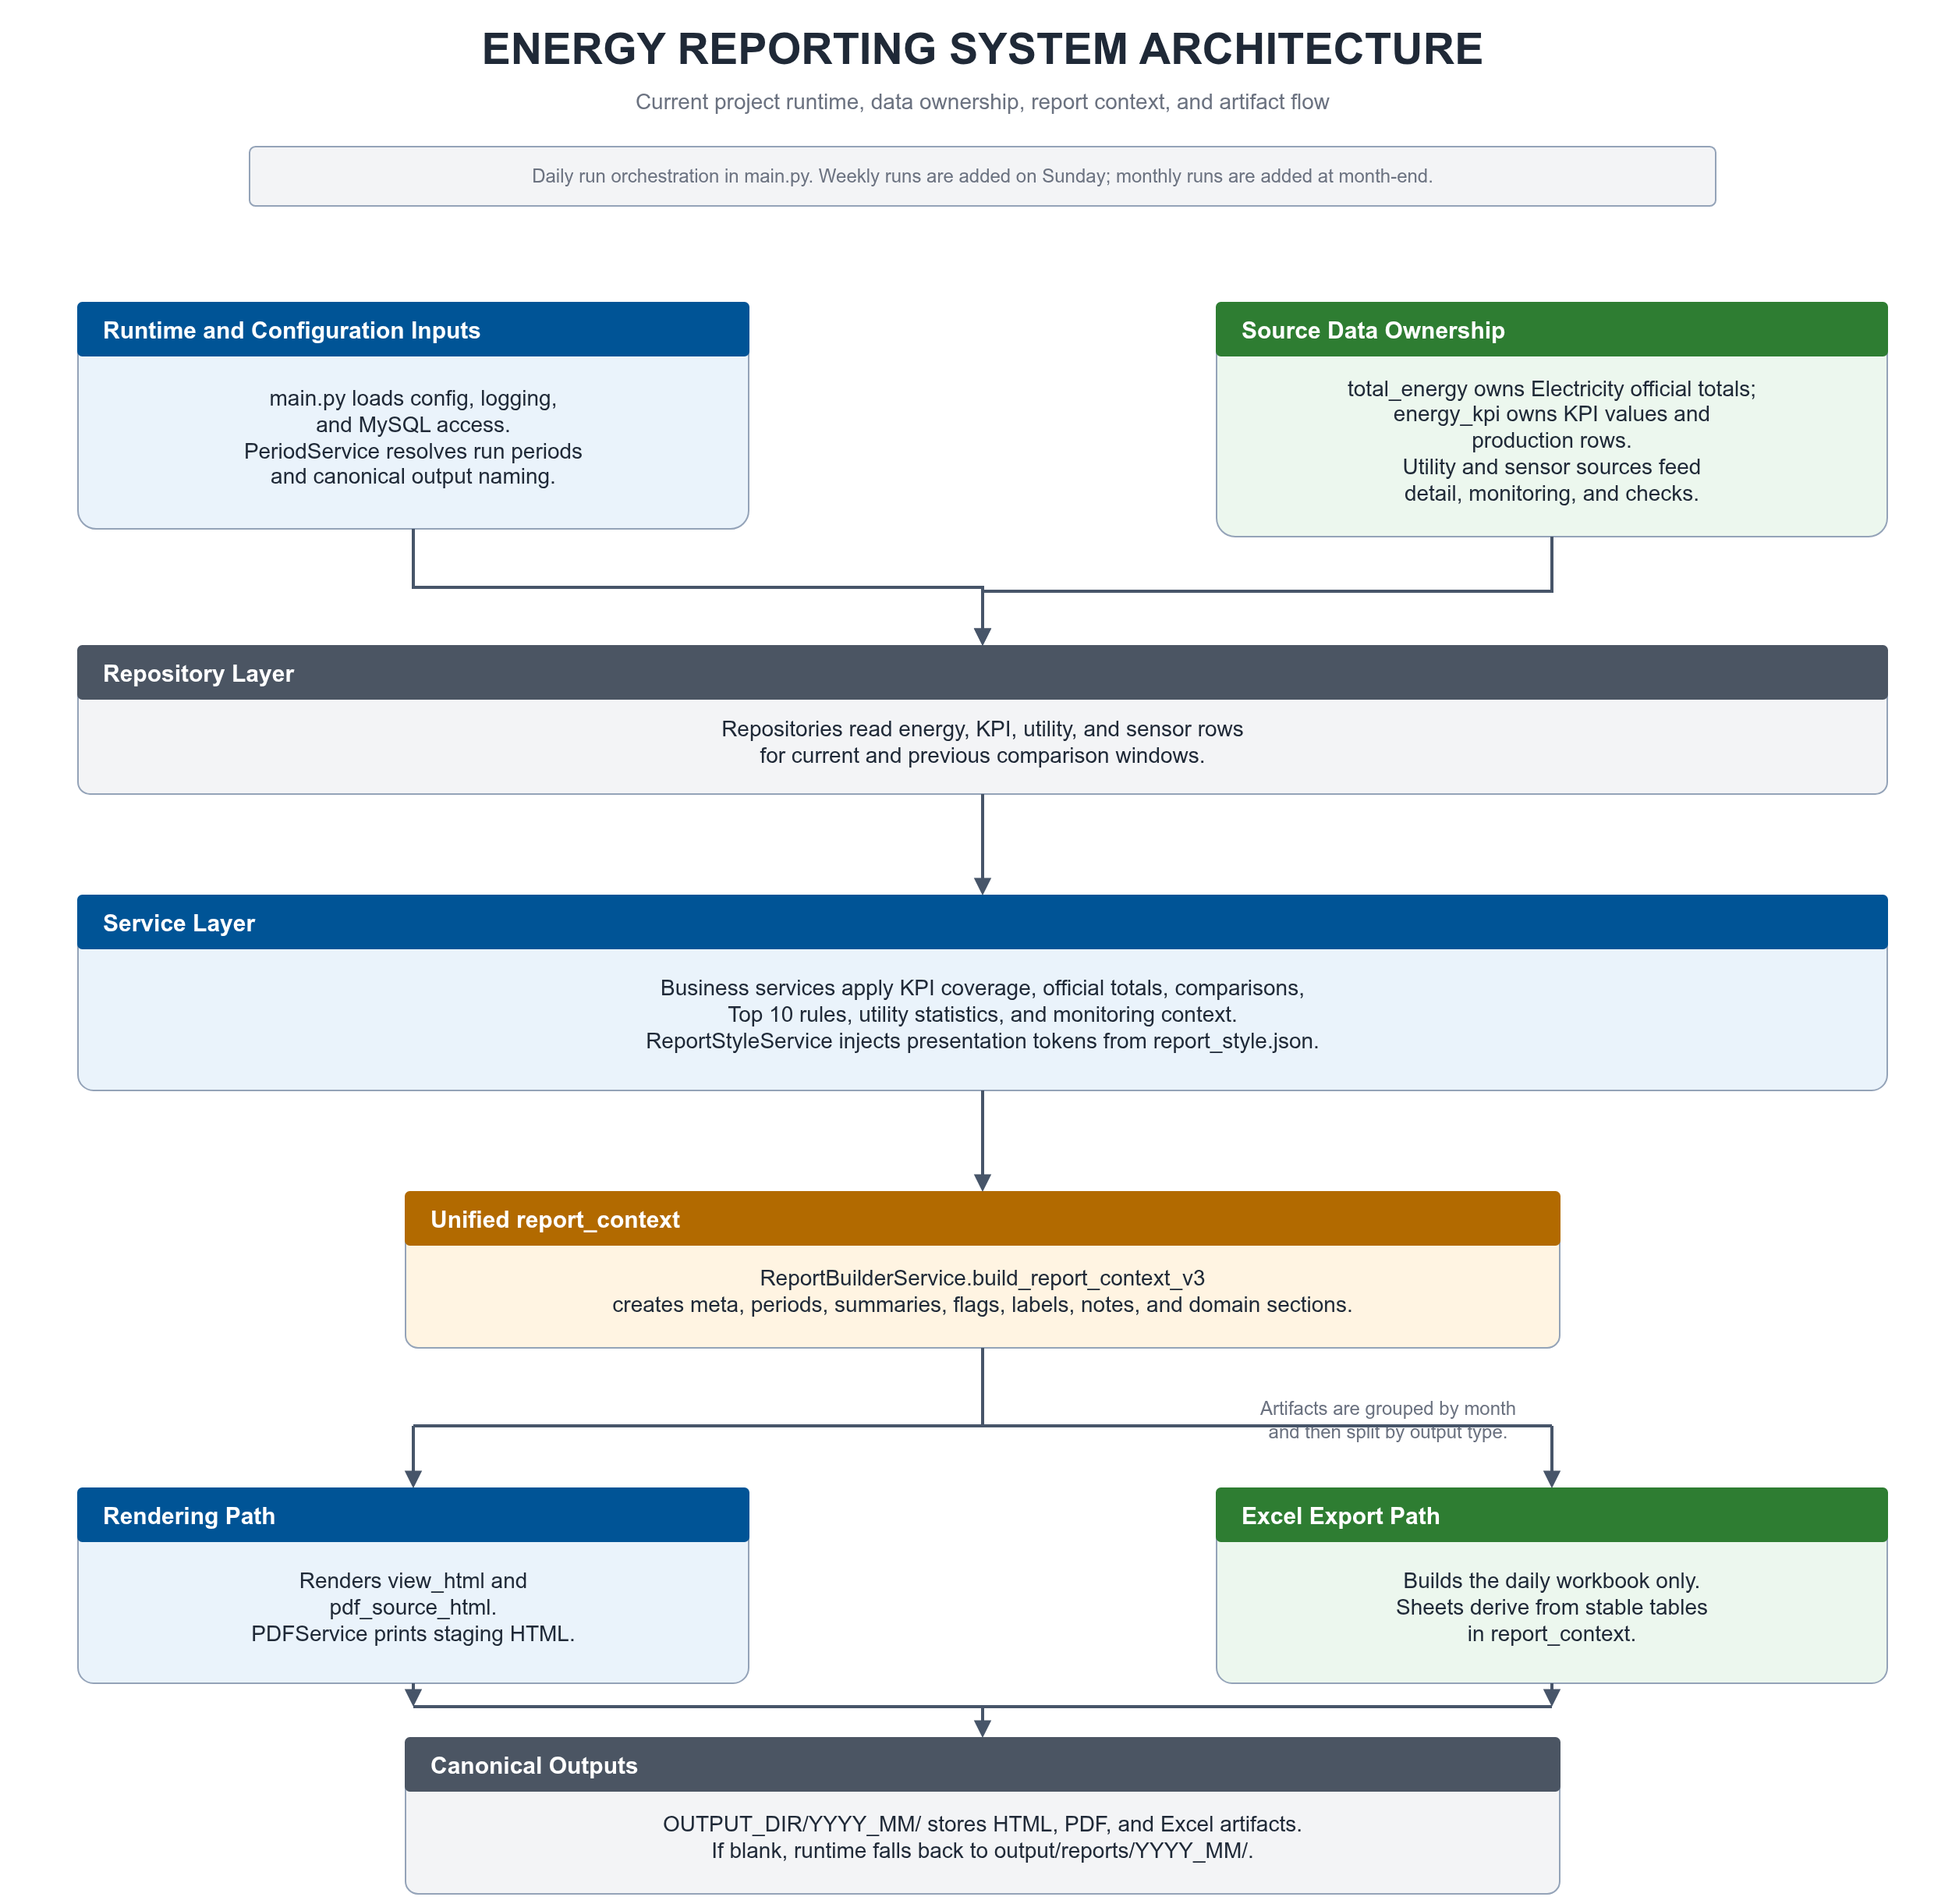
\includegraphics[width=\textwidth]{figure/hinh1_1.png}
	\caption{System architecture of the automated energy reporting pipeline}
	\label{fig:system_architecture}
\end{figure}

Hình \ref{fig:system_architecture} mô tả các lớp chính của hệ thống, bao gồm runtime/configuration inputs, data ownership, repository layer, service layer, report context builder, rendering path, Excel export path, và canonical output structure.

\begin{figure}[H]
	\centering
	% Draw.io source: figure/project_diagrams.drawio, sheet "Report Generation Flow".
	% Export artifact: figure/hinh1_2.png.
	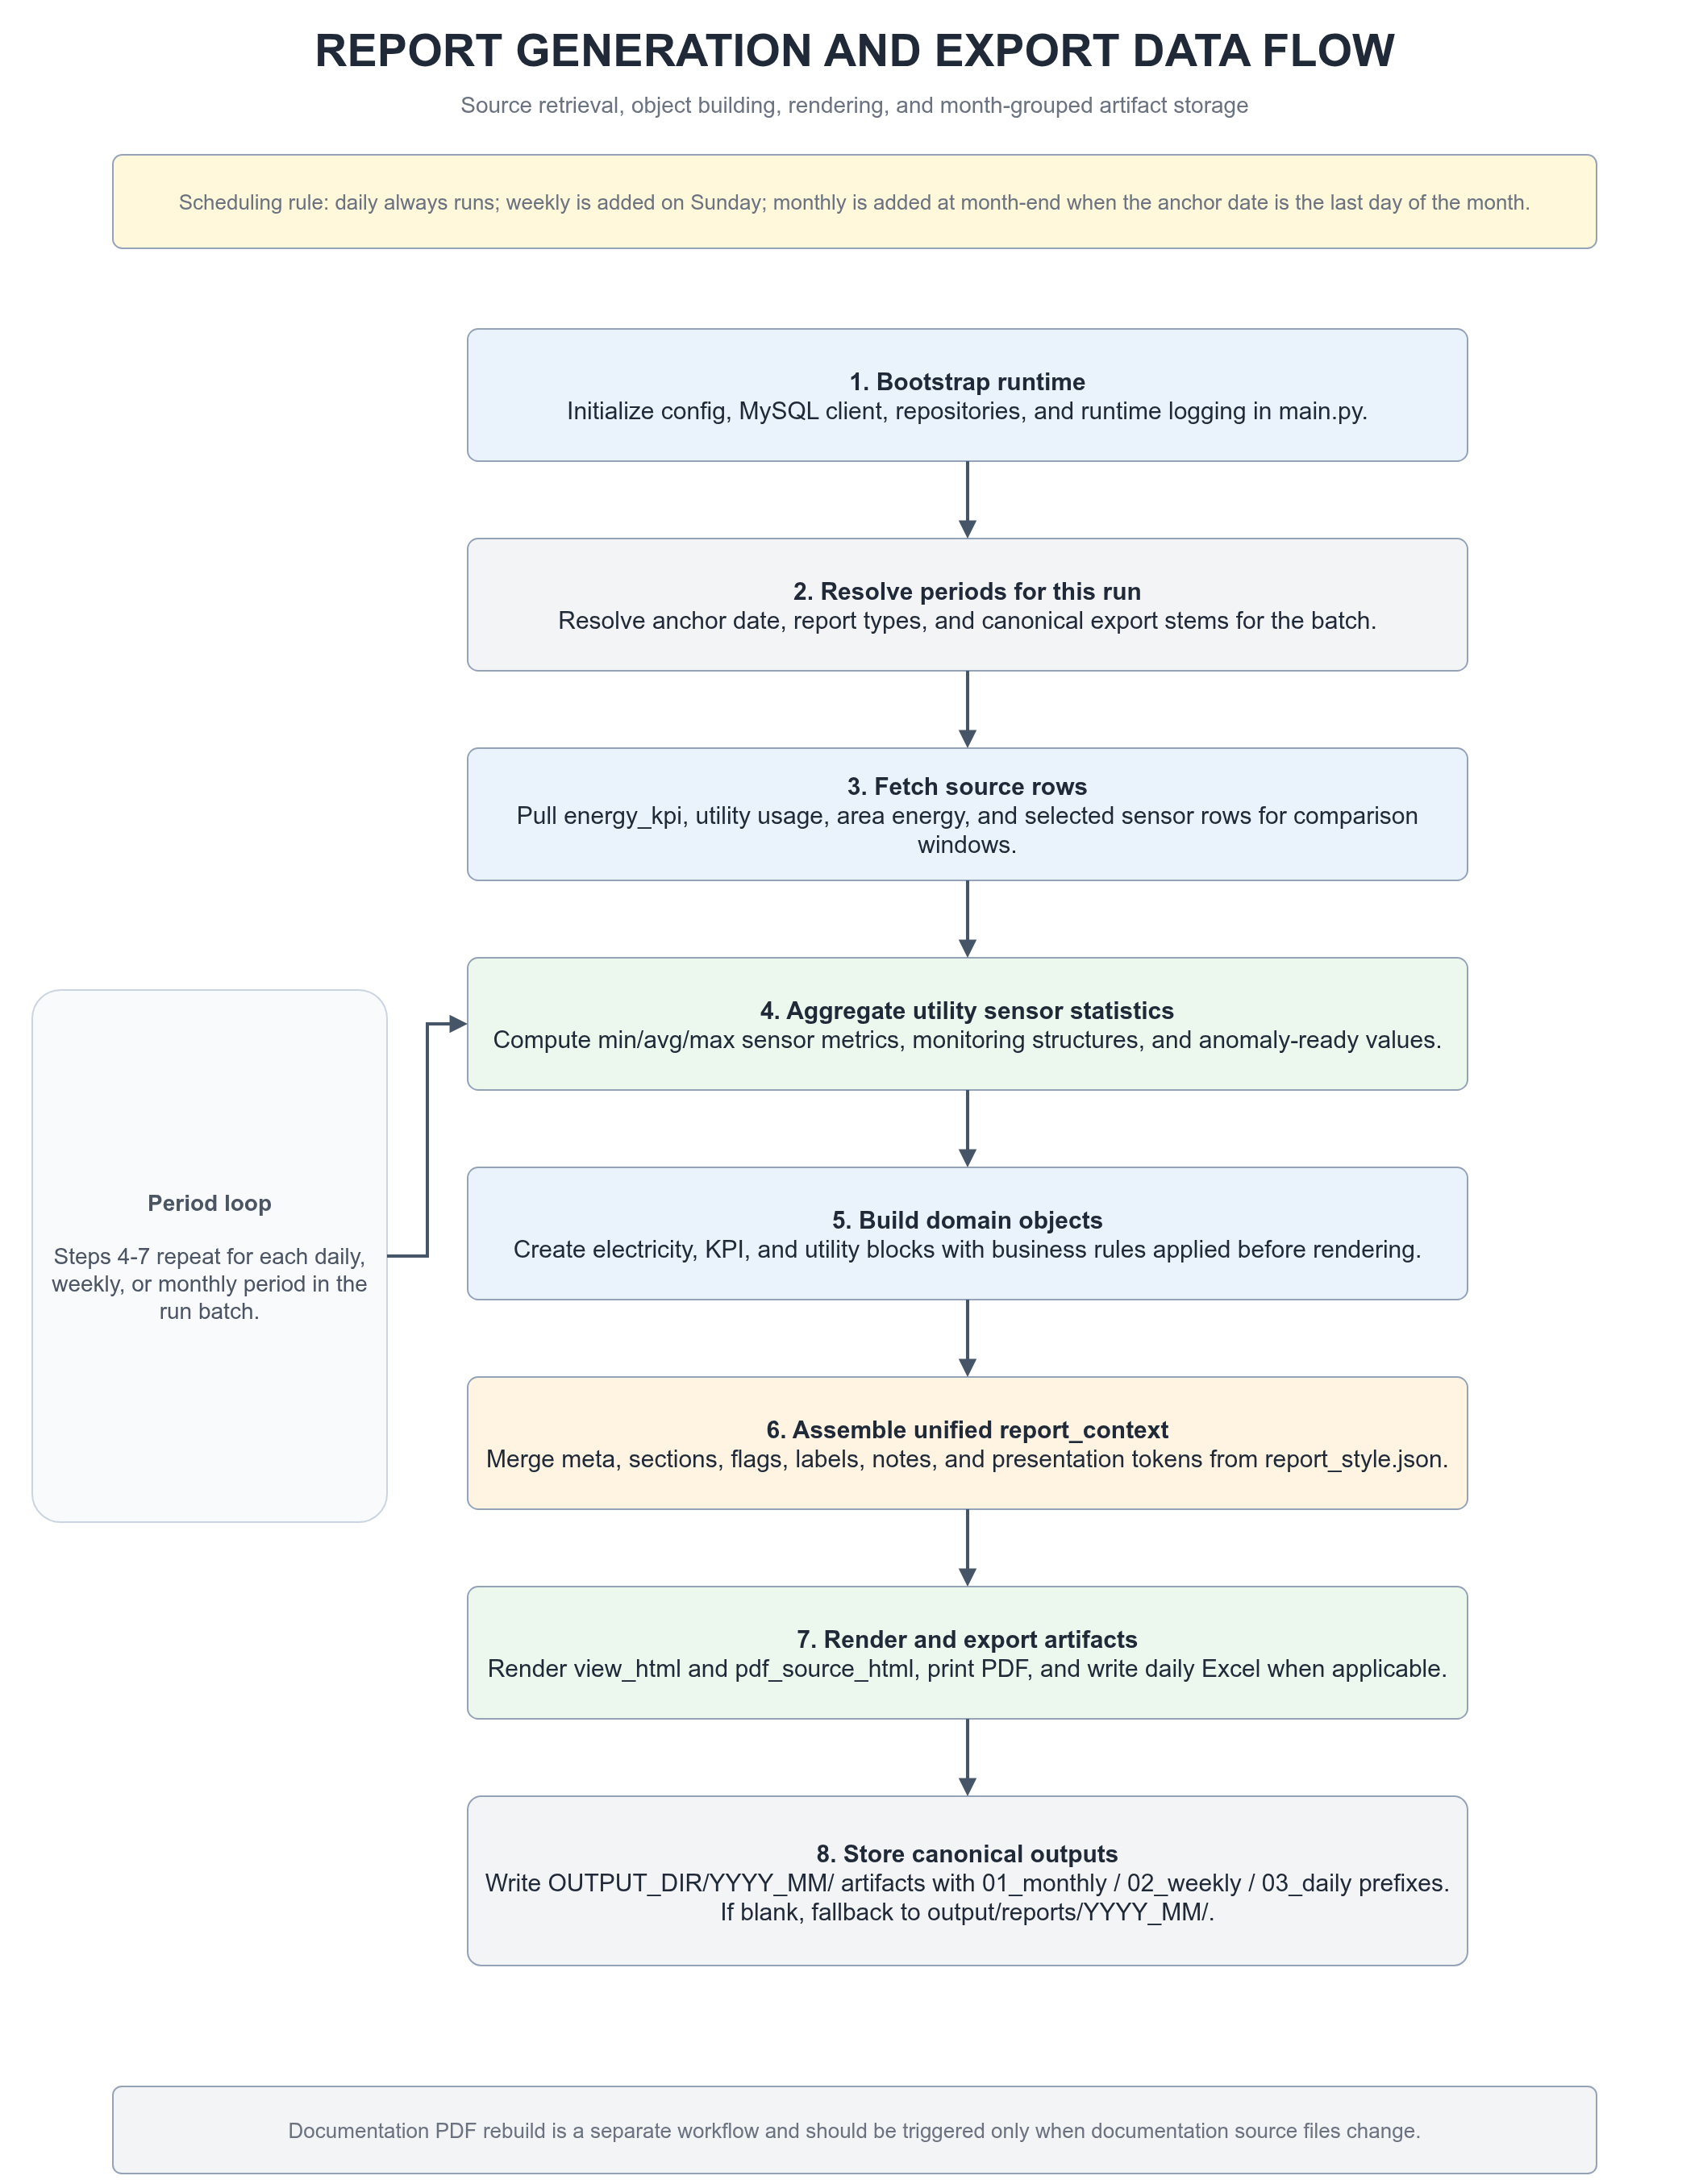
\includegraphics[width=\textwidth]{figure/hinh1_2.png}
	\caption{Report generation and export data flow for the current project runtime}
	\label{fig:report_generation_flow}
\end{figure}

Hình \ref{fig:report_generation_flow} mô tả chu trình thực thi từ bước load config, resolve scheduled periods, fetch source rows, aggregate sensor statistics, build domain objects, assemble \texttt{report\_context}, render artifacts, đến lưu output theo cấu trúc tháng.

\clearpage

\section{Ma trận thành phần chính}

Bảng \ref{tab:component_matrix} là ví dụ về cách trình bày một bảng kỹ thuật ngắn gọn, tập trung vào trách nhiệm chính và output của từng domain.

\begin{table}[htbp]
	\centering
	\renewcommand{\arraystretch}{1.3}
	\caption{Project component matrix for the energy reporting system}
	\label{tab:component_matrix}
	\begin{tabularx}{\linewidth}{|>{\RaggedRight\arraybackslash}p{3.0cm}|>{\RaggedRight\arraybackslash}X|>{\RaggedRight\arraybackslash}X|}
		\hline
		\textbf{Component} & \textbf{Primary Responsibility} & \textbf{Typical Output} \\ \hline
		Electricity domain & Official totals, area totals, comparison blocks, Top 10 meters, and detail tables & HTML sections, PDF sections, Excel detail sheets \\ \hline
		Utility domain & Utility consumption, utility energy, sensor monitoring, and anomaly-ready summaries & HTML/PDF tables, sensor monitoring cards, Excel utility sheets \\ \hline
		KPI domain & Coverage-first KPI context, production linkage, variance analysis, and comparison charts & KPI summary cards, matrices, detail blocks, charts \\ \hline
		Export workflow & Render view HTML, PDF source HTML, PDF, and daily Excel workbook with canonical naming & Month-grouped output artifacts under the project output tree \\ \hline
		Documentation workflow & Maintain project technical documentation, rebuild PDF when docs change, and preserve release-ready references & Versioned technical PDF under \texttt{docs/output/} \\ \hline
	\end{tabularx}
\end{table}

\section{Quy tắc nghiệp vụ và nguyên tắc tính toán}

Các tài liệu kỹ thuật trong dự án nên mô tả rõ các nguyên tắc cốt lõi sau:

\begin{enumerate}[label=-]
\item \textbf{Source of truth}: \texttt{energy\_kpi} là nguồn chính thức cho KPI reporting và official energy totals.
\item \textbf{Coverage-first KPI logic}: không prorate KPI blocks và luôn ưu tiên kỳ có coverage hợp lệ.
\item \textbf{Missing vs zero}: giá trị bằng 0 là dữ liệu hợp lệ, còn dữ liệu thiếu phải được thể hiện rõ ràng.
\item \textbf{Dense period rendering}: các bảng theo ngày hoặc theo kỳ phải render đủ các mốc cần thiết, không bỏ sót hàng chỉ vì thiếu giá trị.
\item \textbf{Backend-first business logic}: business rules nằm ở service/backend layer, không nhân bản logic trong template.
\item \textbf{Output consistency}: view HTML, PDF source HTML, PDF, và Excel phải bám cùng report context và cùng naming convention đã được chấp nhận.
\end{enumerate}

Các nguyên tắc vận hành năng lượng và quản lý hệ thống năng lượng như ISO 50001 là nguồn tham chiếu phù hợp khi xây dựng các mô tả ở mức policy hoặc quản trị tổng thể \cite{ref_iso50001}.

\section{Ví dụ công thức KPI}

Một ví dụ đơn giản nhưng sát ngữ cảnh dự án là công thức intensity-based KPI:

\begin{equation}
	\text{Energy Intensity} = \frac{\text{Total Energy Consumption}}{\text{Production Output}}
	\label{eq:energy_intensity}
\end{equation}

Công thức \ref{eq:energy_intensity} nên chỉ được áp dụng khi cả hai thành phần năng lượng và sản lượng đều có coverage hợp lệ và đáp ứng business rule của kỳ báo cáo.

\begin{tabular}{|p{0.5cm}|l|l|}
	\hline
	& $\text{Total Energy Consumption}$ &: Tổng năng lượng của kỳ báo cáo;\\ \hline
	& $\text{Production Output}$ &: Sản lượng hợp lệ của cùng kỳ;\\ \hline
	& $\text{Energy Intensity}$ &: Chỉ số năng lượng trên đơn vị sản lượng.\\ \hline
\end{tabular}

Khi tài liệu mô tả các công thức cụ thể hơn, nên nêu kèm điều kiện áp dụng, quy tắc coverage, và các trường hợp không được tính để tránh hiểu sai logic implementation.

\section{Workflow cập nhật tài liệu và phát hành PDF}

Workflow khuyến nghị cho subsystem tài liệu kỹ thuật là:

\begin{enumerate}[label=-]
\item cập nhật source Markdown hoặc LaTeX liên quan đến project documentation;
\item kiểm tra lại hình, biểu đồ, tài liệu tham khảo, và các file \texttt{\textbackslash input};
\item build lại PDF bằng \texttt{latexmk + XeLaTeX + biber};
\item kiểm tra PDF đầu ra trong \texttt{docs/output/};
\item chỉ phát hành hoặc chia sẻ khi nội dung tài liệu khớp với trạng thái implementation và naming rules hiện tại.
\end{enumerate}

Đối với project này, PDF không cần rebuild cho mọi thay đổi code. PDF chỉ cần rebuild khi các source tài liệu, hình minh họa, tài liệu tham khảo, hoặc workflow/rules của documentation thay đổi. Cách tiếp cận này phù hợp với mục tiêu giữ tài liệu luôn đồng bộ mà không tạo thêm noise không cần thiết trong pipeline vận hành.

\section{Kiểm soát thay đổi và checklist phát hành}

Trước khi phát hành một bản technical PDF mới, nên rà soát tối thiểu các hạng mục sau:

\begin{enumerate}[label=-]
\item tên tài liệu, phạm vi, và phiên bản tài liệu;
\item tính nhất quán giữa nội dung mô tả và code hiện tại;
\item tính đúng đắn của business rules và KPI calculation notes;
\item tính hợp lệ của figures, tables, cross references, và bibliography;
\item output naming và vị trí lưu file PDF;
\item việc có hay không cần cập nhật checklist, runbook, hoặc project status song song với tài liệu PDF.
\end{enumerate}

\section{Current handover-readiness snapshot}

Ở trạng thái hiện tại, bộ technical manual đã có một cấu trúc đủ rõ để dùng cho internal handover review. Chapter order hiện hành gồm:

\begin{enumerate}[label=-]
\item document metadata và revision history;
\item project overview và phạm vi tài liệu;
\item data sources và repository / service mapping;
\item business rules và KPI reporting rules;
\item output structure và release workflow;
\item deployment and operations;
\item troubleshooting;
\item glossary và naming conventions dưới dạng appendix.
\end{enumerate}

Các thành phần trên đã tạo được một luồng đọc hợp lý từ governance, sang architecture, data ownership, business rules, vận hành, và cuối cùng là lớp tra cứu thuật ngữ. Điều này phù hợp với mục tiêu dùng bộ PDF như một tài liệu kỹ thuật có thể review, handover, và đối chiếu với runtime thật.

Ở góc nhìn readiness, các điểm đã đủ tốt cho internal review gồm:

\begin{enumerate}[label=-]
\item chapter order đã ổn định và không còn mang tính lecture-template;
\item glossary appendix đã tồn tại thật, không còn ở trạng thái placeholder;
\item revision history đã phản ánh các checkpoint chính của subsystem LaTeX;
\item output structure, deployment baseline, naming conventions, và PDF rebuild rules đã được mô tả rõ;
\item generated technical PDFs đã được rebuild và verify sau các lần cập nhật chính.
\end{enumerate}

Các điểm còn mở trước khi xem tài liệu là approved handover baseline gồm:

\begin{enumerate}[label=-]
\item gán reviewer chính thức cho bản technical manual;
\item chốt approver hoặc sign-off owner;
\item sau vòng review nội bộ, cân nhắc freeze một version ổn định hơn như \texttt{v1.0} nếu không còn thay đổi lớn về cấu trúc.
\end{enumerate}

\section{Documentation maintenance checklist}

Checklist tối thiểu để duy trì bộ tài liệu ở trạng thái usable và không drift khỏi implementation là:

\begin{enumerate}[label=-]
\item xác nhận phạm vi update của tài liệu;
\item xác nhận các screenshot, sơ đồ, bảng biểu, và examples phản ánh đúng implementation hiện tại;
\item rà lại business rules, KPI formulas, output naming, và source-of-truth notes nếu thay đổi có chạm vào domain logic;
\item build lại PDF và kiểm tra \texttt{docs/output/} khi documentation source, figures, references, hoặc workflow rules thay đổi;
\item chỉ chia sẻ hoặc dùng cho review khi nội dung và formatting đã được rà lại đầy đủ.
\end{enumerate}

\noindent\textbf{Operational notes}

\begin{enumerate}[label=-]
\item Technical documentation phải được cập nhật khi docs source thay đổi có ý nghĩa, không để trôi xa implementation.
\item Generated PDFs là output artifacts, không phải primary source.
\item Nếu build lỗi, cần giữ log và báo lỗi rõ thay vì bỏ qua bước rebuild hoặc review PDF.
\end{enumerate}

\section{Tổng kết chương}

Chapter tổng quan này hiện không còn là một chapter mẫu thuần túy. Nó đã trở thành phần mở đầu thực sự của bộ technical manual, mô tả mục tiêu tài liệu, phạm vi, kiến trúc hệ thống, workflow cập nhật docs, và trạng thái handover-readiness hiện tại. Kết hợp với các chapter còn lại và appendix glossary, bộ tài liệu hiện đã ở mức phù hợp cho internal review và gần sẵn sàng cho một baseline handover có kiểm soát.
